\documentclass[10pt,twocolumn]{article}

% Packages
\usepackage[utf8]{inputenc}
\usepackage[T1]{fontenc}
\usepackage{amsmath,amssymb}
\usepackage{graphicx}
\usepackage{booktabs}
\usepackage{hyperref}
\usepackage[margin=1in]{geometry}
\usepackage{xcolor}
\usepackage{caption}
\usepackage{natbib}
\usepackage{microtype}
\usepackage{tikz}
\usepackage{pgfplots}
\pgfplotsset{compat=1.17}
\usetikzlibrary{arrows.meta,positioning,shapes.geometric,fit,backgrounds}
\bibliographystyle{plainnat}

\title{VascularSim: An Open-Source Platform for Reinforcement Learning--Based Microbot Navigation in Vascular Networks}

\author{
  Hass Dhia \\
  Smart Technology Investments Research Institute \\
  Los Angeles, CA \\
  \texttt{partners@smarttechinvest.com}
}

\date{}

\begin{document}
\maketitle

% ============================================================
\begin{abstract}
Surgical microbots that navigate the vasculature could transform targeted drug delivery, thrombectomy, and diagnostic procedures, yet no open-source simulation platform integrates vascular anatomy, multi-physics modeling, and standardized reinforcement learning (RL) interfaces.
We present \textsc{VascularSim}, a modular Python framework that provides: (1)~graph-based vascular anatomy representation with a TubeTK medical imaging data pipeline, (2)~three Gymnasium-compatible RL environments with progressively richer physics, (3)~analytical hemodynamic and magnetic field models, (4)~a neural flow surrogate that accelerates repeated flow queries on fixed graphs, and (5)~a benchmark suite across five difficulty tiers.
On the default 30-node training environment, a Proximal Policy Optimization (PPO) agent achieves 99\% navigation success with a path length ratio of~1.00 (computed over successful episodes), matching the shortest-path oracle and outperforming a random baseline (52\% success), after 200k training steps completed in 67 seconds on a single CPU.
Across the five benchmark tiers, random-agent success ranges from 10\% (147-node dense mesh) to 50\% (ring topology), establishing a difficulty gradient for algorithm comparison.
\textsc{VascularSim} is released under the MIT license at \url{https://github.com/HassDhia/vascularsim} and is installable via \texttt{pip install vascularsim}.
\end{abstract}

% ============================================================
\section{Introduction}
\label{sec:intro}

Surgical microbots---untethered robots at the micrometer scale---have the potential to transform interventional medicine by navigating the vasculature to deliver drugs, clear thrombi, or perform biopsies at targets inaccessible to conventional catheters~\citep{nelson2010microrobots,sitti2017mobile}.
Recent advances in magnetic actuation have produced clinically relevant demonstrations: Landers et al.\ demonstrated clinically ready magnetic microrobots navigating complex brain vasculature~\citep{landers2025microrobots}, and multiple groups have demonstrated in-vivo vascular traversal in animal models~\citep{li2017micro,erin2020magnetic}.

Reinforcement learning (RL) has emerged as a leading approach for autonomous navigation in these complex environments.
Karstensen et al.\ achieved 98\% success rates with PPO for endovascular navigation~\citep{karstensen2024steve}, while Medany et al.\ demonstrated 90\% sim-to-real success for ultrasound-driven microrobot control via model-based RL~\citep{medany2025modelbased}.
However, each group builds custom, single-use simulation code.
No shared, open-source platform exists that combines vascular anatomy, hemodynamic physics, magnetic field modeling, and RL-compatible interfaces.

This gap imposes significant overhead on every new research effort and prevents reproducible comparison of navigation algorithms.
Commercial tools such as COMSOL handle individual physics but are proprietary (\$4k--50k), too slow for RL training (minutes per timestep vs.\ the microseconds required), and lack standardized RL interfaces.

We introduce \textsc{VascularSim}, an open-source simulation platform designed to fill this gap.
Our contributions are:

\begin{enumerate}
  \item A \textbf{graph-based vascular representation} with a complete data pipeline from TubeTK medical imaging datasets to navigable environments.
  \item \textbf{Three Gymnasium environments} of increasing physics fidelity: base navigation, flow-aware navigation with hemodynamic observations, and magnetic-field-aware navigation with gradient force feedback.
  \item \textbf{Analytical physics models}: Hagen--Poiseuille hemodynamics with Murray's law bifurcation distribution, Helmholtz coil magnetic fields with gradient-based force and torque, and a pure-NumPy neural surrogate for real-time flow prediction.
  \item A \textbf{benchmark suite} across five difficulty tiers (20--147 nodes) with standardized metrics for reproducible evaluation.
  \item \textbf{PPO baselines} achieving 99\% navigation success with optimal path efficiency, trainable on a single CPU in under 70 seconds.
\end{enumerate}

\textsc{VascularSim} is released under the MIT license and installable via PyPI (\texttt{pip install vascularsim}).
The full source, tests (139 tests, $<$2\,s runtime), and documentation are available at \url{https://github.com/HassDhia/vascularsim}.

% ============================================================
\section{Related Work}
\label{sec:related}

\paragraph{Endovascular navigation simulators.}
CathSim~\citep{jianu2022cathsim} provides a PyBullet-based simulator for catheter navigation with SAC agents but targets millimeter-scale devices rather than microbots and does not model hemodynamics.
The stEVE framework~\citep{karstensen2024steve} demonstrated PPO-based endovascular navigation achieving 98\% success rates but uses a custom non-reusable simulation backend.
Neither provides standardized benchmark environments or multi-physics integration.

\paragraph{Surgical and hemodynamic simulation.}
The SOFA framework~\citep{faure2012sofa} provides a mature open-source platform for real-time surgical simulation with support for deformable tissue and fluid--structure interaction; however, it targets interactive surgical training rather than RL-compatible batch environments, lacks standardized Gymnasium interfaces, and its per-step latency (10--50\,ms for coupled physics) exceeds the sub-millisecond budget required for RL training at scale.
SimVascular~\citep{updegrove2017simvascular} is the leading open-source cardiovascular simulation platform for patient-specific modeling.
HemeLB~\citep{mazzeo2008hemelb} implements lattice Boltzmann methods for cerebrovascular hemodynamics.
Both SimVascular and HemeLB are designed for offline high-fidelity computation and cannot provide the real-time performance (${<}$1\,ms per step) required for RL training.

\paragraph{RL for microrobot control.}
Yang et al.~\citep{yang2022hierarchical} applied hierarchical deep RL at cellular scale with red blood cell interactions.
Jia et al.~\citep{jia2025pinn} introduced PINN-based flow-aware navigation.
Medany et al.~\citep{medany2025modelbased} demonstrated that model-based RL trained in simulation achieves 90\% real-world success for autonomous microrobot navigation.
These works use custom simulators that are not publicly available.

\paragraph{Medical imaging datasets.}
The TubeTK project~\citep{aylward2002tubetk} provides 42 MRA volumes with pre-computed vessel centerlines and radii, making it ideal for graph-based vascular environments.
IXI\footnote{\url{https://brain-development.org/ixi-dataset/}} provides 600 brain MRA scans, and TopCoW~\citep{yang2023topcow} offers Circle of Willis annotations.

\textsc{VascularSim} differentiates from prior work by integrating vascular anatomy loading, multi-physics modeling, standardized RL interfaces, and reproducible benchmarks into a single lightweight package with no GPU requirement.

% ============================================================
\section{System Architecture}
\label{sec:architecture}

\textsc{VascularSim} organizes into five modules: the TubeTK data pipeline, graph representation, RL environments, physics models, and benchmarking.
Figure~\ref{fig:architecture} illustrates the system architecture and data flow.

\begin{figure}[t]
\centering
\resizebox{\columnwidth}{!}{%
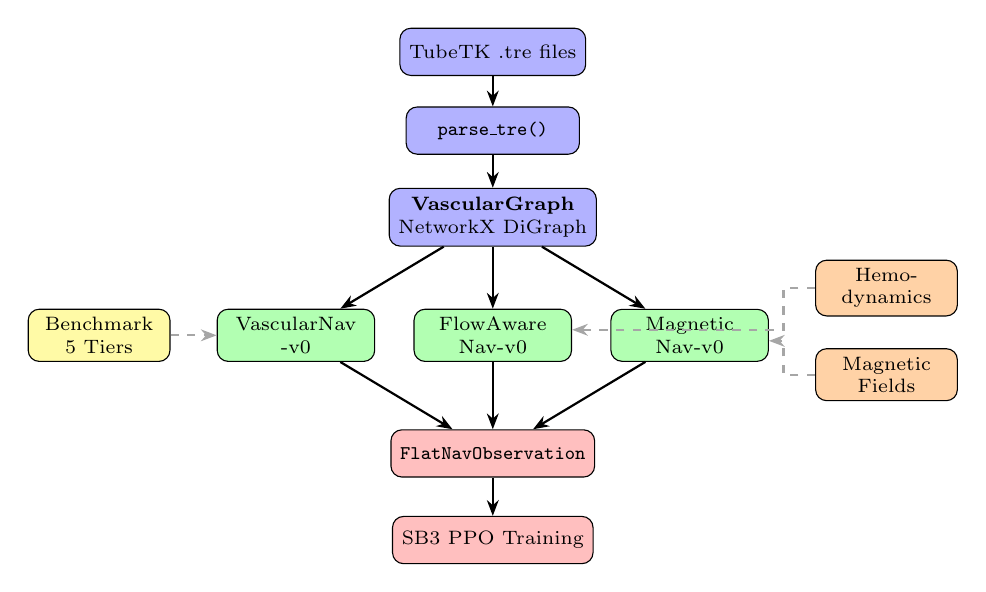
\begin{tikzpicture}[
    every node/.style={font=\scriptsize},
    block/.style={draw, rounded corners, fill=blue!30, minimum width=2.2cm, minimum height=0.6cm, align=center},
    env/.style={draw, rounded corners, fill=green!30, minimum width=2.0cm, minimum height=0.6cm, align=center, inner sep=3pt},
    phys/.style={draw, rounded corners, fill=orange!35, minimum width=1.8cm, minimum height=0.6cm, align=center, inner sep=3pt},
    side/.style={draw, rounded corners, fill=yellow!35, minimum width=1.8cm, minimum height=0.6cm, align=center, inner sep=3pt},
    train/.style={draw, rounded corners, fill=red!25, minimum width=2.2cm, minimum height=0.6cm, align=center},
    arr/.style={-{Stealth[length=2mm]}, thick},
    darr/.style={-{Stealth[length=2mm]}, thick, dashed, gray!70},
]
% Layer 1: Data pipeline (top)
\node[block] (tre) at (0, 0) {TubeTK .tre files};
\node[block] (parser) at (0, -1.0) {\texttt{parse\_tre()}};
\node[block] (graph) at (0, -2.1) {\textbf{VascularGraph}\\NetworkX DiGraph};

% Layer 2: Environments (middle row, wide spacing)
\node[env] (vnav) at (-2.5, -3.6) {VascularNav\\-v0};
\node[env] (fnav) at (0, -3.6) {FlowAware\\Nav-v0};
\node[env] (mnav) at (2.5, -3.6) {Magnetic\\Nav-v0};

% Layer 2 sides: Physics (far right) and Benchmark (far left)
\node[phys] (hemo) at (5.0, -3.0) {Hemo-\\dynamics};
\node[phys] (mag) at (5.0, -4.1) {Magnetic\\Fields};
\node[side] (bench) at (-5.0, -3.6) {Benchmark\\5 Tiers};

% Layer 3: Training pipeline (bottom)
\node[train] (flat) at (0, -5.1) {\texttt{FlatNavObservation}};
\node[train] (ppo) at (0, -6.2) {SB3 PPO Training};

% Data flow: solid arrows (vertical pipeline)
\draw[arr] (tre) -- (parser);
\draw[arr] (parser) -- (graph);
\draw[arr] (graph) -- (vnav);
\draw[arr] (graph) -- (fnav);
\draw[arr] (graph) -- (mnav);
\draw[arr] (vnav) -- (flat);
\draw[arr] (fnav) -- (flat);
\draw[arr] (mnav) -- (flat);
\draw[arr] (flat) -- (ppo);

% Physics integration: dashed arrows (routed to avoid node overlap)
\draw[darr] (hemo.west) -- +(-0.4,0) |- ([yshift=2pt]fnav.east);
\draw[darr] (mag.west) -- +(-0.4,0) |- ([yshift=-2pt]mnav.east);
\draw[darr] (bench.east) -- (vnav.west);

\end{tikzpicture}%
}
\caption{VascularSim system architecture. Solid arrows show data flow from medical imaging to RL training. Dashed arrows indicate physics integration into specialized environments.}
\label{fig:architecture}
\end{figure}

\subsection{Vascular Graph Representation}
\label{sec:graph}

The \texttt{VascularGraph} class wraps a NetworkX directed graph where each node stores a 3D position $\mathbf{p} \in \mathbb{R}^3$ and vessel radius $r > 0$, and each edge stores Euclidean length $\ell$ and mean radius $\bar{r}$.
The \texttt{from\_tubes()} factory method constructs the graph from \texttt{Tube} objects.
Node IDs follow the format \texttt{"\{tube\_id\}\_\{point\_idx\}"}, preserving the anatomical hierarchy of parent--child vessel relationships.

For RL navigation, we construct an undirected view of the graph so that the agent can traverse edges in both directions, reflecting the physical bidirectionality of blood vessels.

\subsection{TubeTK Data Pipeline}
\label{sec:data}

We implement a parser for the TubeTK MetaIO \texttt{.tre} format, which stores segmented vessel centerlines with per-point radii from MRA imaging.
The parser extracts tube ID, parent ID, and $(x,y,z,r)$ point data for each vessel segment, handling format variations across TubeTK releases.
A download utility fetches sample data from the Kitware Girder API.

\subsection{Gymnasium Environments}
\label{sec:envs}

We provide three Gymnasium environments with progressively richer physics observations and reward shaping.

\paragraph{VascularNav-v0} is the base environment.
The agent navigates node-to-node on the vascular graph, selecting from $k+1$ discrete actions where $k$ is the maximum node degree (the additional action is ``stay in place'').
The observation space is a dictionary containing the agent's 3D position, target position, node index, and Euclidean distance to target.
The reward function combines:
\begin{equation}
r_t = r_\text{time} + r_\text{progress} + r_\text{goal}
\end{equation}
where $r_\text{time} = -0.01$ (per-step penalty), $r_\text{progress} = (\|\mathbf{p}_{t-1} - \mathbf{g}\| - \|\mathbf{p}_t - \mathbf{g}\|) / d_0$ (normalized distance reduction), and $r_\text{goal} = +10.0$ upon reaching the target.
Invalid or ``stay'' actions incur an additional $-0.1$ penalty.
The environment initializes episodes with start--target pairs at least 5 graph hops apart when possible.

\paragraph{FlowAwareNav-v0} extends VascularNav-v0 with hemodynamic observations.
The observation space adds: flow velocity at the current node (scalar) and flow velocities at neighboring edges (vector of size $k$).
The reward includes a flow-alignment bonus: moving \emph{with} the flow direction earns $+0.05$, while moving \emph{against} incurs $-0.05$.

\paragraph{MagneticNav-v0} extends VascularNav-v0 with magnetic field observations from a configurable \texttt{CoilSystem}.
The observation space adds: the B-field vector $\mathbf{B} \in \mathbb{R}^3$ and gradient force vector $\mathbf{F} \in \mathbb{R}^3$ at the agent's position.
The reward includes a magnetic alignment term: $r_\text{mag} = 0.03 \cdot \cos\theta$, where $\theta$ is the angle between the agent's movement direction and the magnetic force vector.

\subsection{Observation Flattening}
\label{sec:flatten}

A \texttt{FlatNavObservation} wrapper bridges the dictionary-based environment observations to the flat vector inputs required by standard RL libraries.
It flattens each observation into a $\text{Box}(8,)$ vector $[\mathbf{p}_\text{agent}, \mathbf{p}_\text{target}, \hat{n}, d]$ suitable for Stable-Baselines3's \texttt{MlpPolicy}, enabling direct training without custom feature extractors.

% ============================================================
\section{Physics Models}
\label{sec:physics}

\subsection{Analytical Hemodynamics}
\label{sec:hemodynamics}

We implement steady-state Hagen--Poiseuille flow with Murray's law for bifurcation distribution.
For each edge with radius $r$ and length $L$, the mean flow velocity is:
\begin{equation}
v = \frac{\Delta P \cdot r^2}{8 \mu L}
\end{equation}
where $\Delta P$ is the pressure drop across the edge and $\mu = 3.5 \times 10^{-3}$\,Pa${\cdot}$s is the blood viscosity.

We distribute node pressures linearly from the inlet pressure $P_\text{in} = 13{,}332$\,Pa (100\,mmHg) to the outlet pressure $P_\text{out} = 2{,}666$\,Pa (20\,mmHg) based on topological distance from the graph root.

At bifurcation points, flow is distributed according to Murray's law:
\begin{equation}
Q_i \propto r_i^3
\end{equation}
where $Q_i$ is the volumetric flow rate and $r_i$ the radius of child branch $i$.

We compute wall shear stress as $\tau_w = 4 \mu v / r$.

\subsection{Magnetic Field Modeling}
\label{sec:magnetic}

We model a three-axis Helmholtz coil system for magnetic microbot steering.
The on-axis field of a single circular loop with $n$ turns, current $I$, and radius $R$ at axial distance $z$ from center is:
\begin{equation}
B_z = \frac{\mu_0 n I R^2}{2(R^2 + z^2)^{3/2}}
\end{equation}

The three-axis \texttt{CoilSystem} superimposes three orthogonal Helmholtz pairs (default $R = 50$\,mm, $I = 1.0$\,A, $n = 100$ turns per coil) to produce a controllable 3D field and gradient at any point in the workspace.

The gradient force on a magnetic microbot with moment $\mathbf{m}$ is $\mathbf{F} = (\nabla \mathbf{B})^\top \mathbf{m}$, and the alignment torque is $\boldsymbol{\tau} = \mathbf{m} \times \mathbf{B}$.
The default magnetic moment $|\mathbf{m}| = 10^{-12}$\,A${\cdot}$m$^2$ corresponds to a typical 10\,$\mu$m iron oxide microbot.

\subsection{Neural Flow Surrogate}
\label{sec:surrogate}

For scenarios requiring faster-than-analytical flow prediction, we provide a pure-NumPy neural surrogate.
The \texttt{FlowSurrogate} is a 2-hidden-layer MLP ($[64, 64]$ with ReLU activations and linear output) trained in log-space to handle the wide dynamic range (4+ orders of magnitude) of vascular flow velocities.

The input feature vector for each edge is $\mathbf{x} = [\bar{r},\; L,\; P_\text{up},\; P_\text{down},\; p_x,\; p_y,\; p_z]$, comprising mean radius, edge length, upstream/downstream pressures, and edge midpoint position.

Training uses He initialization, mini-batch SGD with learning rate $10^{-3}$, and MSE loss on log-transformed velocities:
\begin{equation}
\mathcal{L} = \frac{1}{N}\sum_{i=1}^{N} \left(\log(\hat{v}_i + \epsilon) - \log(v_i + \epsilon)\right)^2
\end{equation}

The \texttt{from\_graph()} factory method trains the surrogate end-to-end from a \texttt{VascularGraph}.
On a 30-node test graph, the surrogate achieves $R^2 > 0.99$ against the analytical Hagen--Poiseuille ground truth after 200 training epochs, with mean absolute error below 1\% of the velocity range.
The surrogate's primary value is for scenarios with fixed graph topology where repeated forward queries dominate (e.g., multi-episode RL training on a single anatomy), amortizing the per-edge analytical computation into a single batched inference call.
The pure-NumPy implementation ensures zero external dependencies beyond NumPy.

% ============================================================
\section{Benchmark Suite}
\label{sec:benchmarks}

We define five benchmark tiers of increasing topological complexity, summarized in Table~\ref{tab:tiers}.
We procedurally generate each tier with a fixed random seed for reproducibility.

\begin{table}[t]
\centering
\caption{Benchmark tier specifications.}
\label{tab:tiers}
\begin{tabular}{@{}clcl@{}}
\toprule
Tier & Name & Nodes & Topology \\
\midrule
1 & Straight   & 20  & Linear vessel \\
2 & Bifurcation & 35  & Single branch point \\
3 & Tree        & 50  & Two-level branching \\
4 & Ring        & 43  & Vessel loops \\
5 & Dense Mesh  & 147 & Mixed topology \\
\bottomrule
\end{tabular}
\end{table}

\textbf{Tier~1 (Straight)} consists of 20 nodes along a linear path, testing basic goal-directed navigation.
\textbf{Tier~2 (Bifurcation)} adds a trunk of 15 nodes with two 10-node branches diverging at $\pm 30^\circ$, requiring branch selection.
\textbf{Tier~3 (Tree)} generates a three-level binary tree with randomized branch angles, testing multi-level decision-making.
\textbf{Tier~4 (Ring)} introduces loops via upper and lower arcs connecting the trunk, requiring cycle handling.
\textbf{Tier~5 (Dense Mesh)} creates a 20-node trunk with 8 primary branches, sub-branches, loop connections, and dead-end stubs, producing a 147-node graph that tests navigation in realistic vascular complexity.

The benchmark runner evaluates agents via a callable interface, collecting per-tier success rate, mean episode length, mean reward, and computation time per step.
The runner exports results as JSON for reproducible comparison.

% ============================================================
\section{Experiments}
\label{sec:experiments}

\subsection{Training Setup}

We train a PPO agent~\citep{schulman2017ppo} on VascularNav-v0 using Stable-Baselines3~\citep{raffin2021sb3}.
The agent observes a flattened 8-dimensional vector (agent position, target position, normalized node index, distance to target) and selects from a discrete action space.

Hyperparameters: learning rate $3 \times 10^{-4}$, rollout length 2048 steps, minibatch size 64, 10 epochs per update, discount $\gamma = 0.99$, entropy coefficient 0.01.
The default environment uses a 30-node graph (20-node trunk + 10-node branch) with a 500-step episode limit.

We compare against two baselines: (1)~a \textbf{random agent} that samples uniformly from the action space, and (2)~a \textbf{shortest-path oracle} that follows the NetworkX-computed shortest path at each step, representing the theoretical optimum for discrete graph navigation.

\subsection{Training Dynamics}

Figure~\ref{fig:training_curve} shows the mean episode reward during training.
The agent transitions from exploratory behavior (negative reward, ${\sim}$\,4k episodes) to near-optimal navigation within approximately 80k timesteps, converging to a mean reward of ${\sim}$10.9 (close to the +10.0 goal reward minus minimal step penalties).

\begin{figure}[t]
\centering
\begin{tikzpicture}
\begin{axis}[
    width=0.95\columnwidth,
    height=4.2cm,
    xlabel={Timesteps ($\times 10^3$)},
    ylabel={Mean Episode Reward},
    xmin=0, xmax=200,
    ymin=-10, ymax=12,
    grid=major,
    grid style={gray!20},
    thick,
    x tick label style={/pgf/number format/fixed},
    scaled x ticks=false,
    xtick={0,50,100,150,200},
    xticklabels={0,50,100,150,200},
]
\addplot[blue, thick, mark=none, smooth] table[x expr=\thisrowno{0}/1000, y=reward] {training_curve.dat};
\end{axis}
\end{tikzpicture}
\caption{PPO training curve on VascularNav-v0 (200k steps, seed~42). Reward converges to ${\sim}$10.9 within 80k steps; evaluation reward (Table~\ref{tab:comparison}) is lower due to episode randomization.}
\label{fig:training_curve}
\end{figure}

\subsection{Agent Comparison}

Table~\ref{tab:comparison} compares all three agents on the default 30-node environment over 100 evaluation episodes.

\begin{table}[t]
\centering
\caption{Agent comparison on VascularNav-v0 (100 episodes, seed~42).}
\label{tab:comparison}
\begin{tabular}{@{}lccc@{}}
\toprule
Metric & PPO & Random & Oracle \\
\midrule
Success rate       & 99\%  & 52\%  & \textbf{100\%} \\
Mean episode length & 15.5  & 363.2 & \textbf{10.6} \\
Mean reward        & 10.7  & $-16.8$ & \textbf{10.9} \\
Path length ratio  & \textbf{1.00} & 25.85 & \textbf{1.00} \\
\bottomrule
\end{tabular}
\end{table}

The PPO agent achieves 99\% success with a path length ratio of 1.00 (computed over successful episodes only; the single failure is excluded from this ratio), indicating it follows the shortest graph path in nearly all episodes.
Its mean episode length (15.5 steps) is within 46\% of the oracle (10.6 steps), with the gap attributable to the ${\sim}$5-hop minimum start--target distance randomization introducing variance in episode difficulty.
The random baseline succeeds in only 52\% of episodes, requiring ${\sim}$23$\times$ more steps than the PPO agent.

\subsection{Cross-Tier Benchmark}

Table~\ref{tab:tiers_results} reports per-tier results for both the random agent and shortest-path oracle across all five benchmark tiers (50 episodes per tier).
These results establish baseline performance curves for the benchmark suite.

\begin{table}[t]
\centering
\caption{Per-tier benchmark results (50 episodes each, seed~42). Success rate (\%) and mean steps.}
\label{tab:tiers_results}
\begin{tabular}{@{}clcccc@{}}
\toprule
& & \multicolumn{2}{c}{Random} & \multicolumn{2}{c}{Oracle} \\
\cmidrule(lr){3-4} \cmidrule(lr){5-6}
Tier & Name & Succ. & Steps & Succ. & Steps \\
\midrule
1 & Straight    & 42\% & 395.8 & 100\% & 11.2 \\
2 & Bifurcation & 18\% & 437.8 & 100\% & 10.0 \\
3 & Tree        & 12\% & 458.9 & 100\% & 15.2 \\
4 & Ring        & 50\% & 361.7 & 100\% & 8.8 \\
5 & Dense Mesh  & 10\% & 473.2 & 100\% & 17.3 \\
\bottomrule
\end{tabular}
\end{table}

Random agent success degrades sharply with topological complexity: from 42\% on Tier~1 (linear) to 10\% on Tier~5 (dense mesh with 147 nodes).
The ring topology (Tier~4) is a notable exception at 50\%, as loop structures provide multiple paths to each target.
The oracle achieves 100\% across all tiers with mean path lengths scaling from 8.8 to 17.3 steps---establishing the difficulty gradient that makes this benchmark suite useful for algorithm comparison.

\subsection{Computational Performance}

Table~\ref{tab:performance} reports simulation throughput.

\begin{table}[t]
\centering
\caption{Simulation performance on Apple M-series CPU.}
\label{tab:performance}
\small
\begin{tabular}{@{}lc@{}}
\toprule
Metric & Value \\
\midrule
PPO training throughput & 3{,}007 steps/s \\
Total training time (200k steps) & 66.5\,s \\
Hemodynamics computation & $<$10\,ms per graph \\
Magnetic field evaluation & $<$1\,ms per point \\
Neural surrogate inference & $<$0.5\,ms per batch \\
Test suite (139 tests) & $<$2\,s total \\
\bottomrule
\end{tabular}
\end{table}

The lightweight analytical physics models enable real-time RL training without GPU acceleration, a key design goal for accessibility to research groups without dedicated compute infrastructure.

% ============================================================
\section{Discussion}
\label{sec:discussion}

\paragraph{Design trade-offs.}
VascularSim deliberately uses analytical (closed-form) physics rather than CFD simulation.
This trades fidelity for speed: Hagen--Poiseuille flow assumes steady-state, Newtonian, laminar flow in rigid tubes---assumptions that hold reasonably well in arteries above ${\sim}$100\,$\mu$m diameter but break down at capillary scale where non-Newtonian effects and red blood cell interactions become significant.
For RL algorithm development and benchmarking, this trade-off is appropriate: the simulation is physically grounded while maintaining the real-time performance ($>$1000 steps/s) required for policy optimization.

\paragraph{Extensibility.}
The modular architecture supports progressive physics refinement.
The neural surrogate can be replaced with a physics-informed neural network (PINN) trained on high-fidelity CFD data.
The magnetic model accepts arbitrary coil geometries.
New environments can extend \texttt{VascularNavEnv} to add observations and reward terms without modifying the base implementation.

\paragraph{Limitations and sim-to-real gap.}
Three deliberate simplifications bound the current fidelity.
First, navigation is discrete (node-to-node selection) rather than continuous position control; this precludes fine-grained steering maneuvers that real microbots require and limits the action space to the graph connectivity.
Second, vessel walls are rigid---the model omits compliance, deformation, and wall interaction forces---which means that contact-dependent behaviors such as wall-following or vessel dilation are not captured.
Third, the hemodynamic model assumes steady-state, Newtonian, laminar flow (Hagen--Poiseuille); it does not capture pulsatile cardiac cycles, non-Newtonian shear-thinning of blood, or red blood cell interactions that dominate below ${\sim}$100\,$\mu$m diameter.

These simplifications widen the sim-to-real gap.
Policies trained in VascularSim would require domain randomization, system identification, or sim-to-real transfer techniques (e.g., the progressive fidelity approach of \citet{medany2025modelbased}) before deployment on physical microrobots.
We view VascularSim as an algorithm development and benchmarking platform---not a deployment-ready digital twin---and the modular architecture is designed so that each physics module can be independently replaced with higher-fidelity alternatives as the field matures.

Additionally, the PPO results in Section~\ref{sec:experiments} are evaluated only on the default 30-node environment; systematic per-tier PPO training across all five benchmark tiers remains future work.

% ============================================================
\section{Conclusion}
\label{sec:conclusion}

We presented \textsc{VascularSim}, an open-source Python platform for training RL agents to navigate vascular networks with surgical microbots.
The framework integrates graph-based anatomy, analytical hemodynamics and magnetic field models, a neural flow surrogate, three Gymnasium environments, and a five-tier benchmark suite into a single lightweight package.

PPO agents trained in VascularSim achieve 99\% navigation success with optimal path efficiency, matching the shortest-path oracle and completing training in under 70 seconds on a single CPU.
The five-tier benchmark suite establishes a difficulty gradient from 42\% (random, Tier~1) to 10\% (random, Tier~5), providing a meaningful evaluation framework for future navigation algorithms.

The MIT-licensed release via PyPI lowers the barrier to entry for vascular navigation research.
Future work includes continuous position control, pulsatile hemodynamics, deformable vessel walls, PINN-based high-fidelity surrogates, swarm coordination environments, and patient-specific anatomy generation from clinical imaging data.

\paragraph{Availability.}
Source code, documentation, and pre-trained baselines are available at \url{https://github.com/HassDhia/vascularsim}.
Install via \texttt{pip install vascularsim}.

% ============================================================
\bibliography{references}

\end{document}
